\section{Auswertung}
\label{sec:Auswertung}

\subsection{Untersuchung eines Acrylblocks mit dem A-Scan}
Die Nummerierung der Löcher des Acrylblocks ist in einer Skizze in \autoref{sec:anhang} nachzuschauen.\\
Für den Block wurden mit der Schieblehre die Maße
\begin{eqnarray}
    h &=& 8,04 \mathrm{cm} \nonumber \\
    b &=& 15,04 \mathrm{cm} \nonumber \\
    t &=& 4 \mathrm{cm} \nonumber 
\end{eqnarray}
aufgenommen, wobei $h$ die Höhe, $b$ die Länge und $t$ die Breite des Acrylblocks darstellen. 

Die bei der Regression ermittelten Parameter für Schallgeschwindigkeit $c$ und Anpassungsschichtdicke $d$ lauten
\begin{eqnarray}
    c &=& (2714 \pm 30) \mathrm{m/s} \nonumber \\
    d &=& (4 \pm 1 )\mathrm{mm.} \nonumber 
\end{eqnarray}

Die errechneten Durchmesser der Störstellen sind in \autoref{tab:lochd} zu finden.\\

\begin{table}[h]
    \centering
    \caption{Die errechneten Durchmesser der Störstellen.}
    \begin{tabular}{cc}
      \toprule
      {Lochnummer} & 
      {Durchmesser $d$ in mm }\\
      \midrule
      8  &  6,41    \\
      7  &  5,59    \\
      6  &  4,23    \\
      5  &  3,41    \\
      4  &  3,55    \\
      3  &  3,68    \\
      2  &  3,41    \\
      1  &  30,44   \\
      K1 &  2,18    \\
      K2 &  1,91    \\   
      G  &  10,24   \\
      \bottomrule
    \end{tabular}
    \label{tab:lochd}
  \end{table}
\noindent


\begin{table}[h]
    \centering
    \caption{Die errechneten Tiefen der Störstellen, von unten und von oben.}
    \begin{tabular}{ccc}
      \toprule
      {Lochnummer} & 
      {$s_{unten}$ in mm} &
      {$s_{oben}$ Tiefe in mm} \\
      \midrule
      8  &  6,22  & 1,47  \\
      7  &  5,49  & 2,29  \\
      6  &  4,74  & 3,18  \\
      5  &  4,00  & 4,00  \\
      4  &  3,21  & 4,78  \\
      3  &  2,42  & 5,56  \\
      2  &  1,62  & 6,37  \\
      1  &  0,83  & 4,46  \\
      K1 &  2,07  & 6,05  \\
      K2 &  1,92  & 6,22  \\   
      G  &  5,65  & 1,67  \\
      \bottomrule
    \end{tabular}
 \label{tab:tiefe}
\end{table}
\noindent


\subsection{Untersuchung des Auflösungsvermögens}
Die beiden benachbarten kleinsten Störstellen $K1$ und $K2$ wurden mit beiden verfügbaren
Sonden (1-MHz und 2-MHz) untersucht. Die mit der 1-MHz-Sonde aufgenommenen Messdaten sind in \autoref{fig:1mhz} zu sehen.\\
Mit der 2-MHz-Sonde wurden auch Messwerte aufgenommen, die aber bei der Datenexportation verloren gegangen sind. 
Bei der Aufnahme der Messwerte war zu beobachten, dass die mit der 2-MHz-Sonde erstellte Grafik eher höhere 
Amplituden zeigt, die allerdings schneller ab- und zunehmen, sodass das Signal insgesamt etwas "flackernd"  wirkt.
\begin{figure}[H]
  \centering
  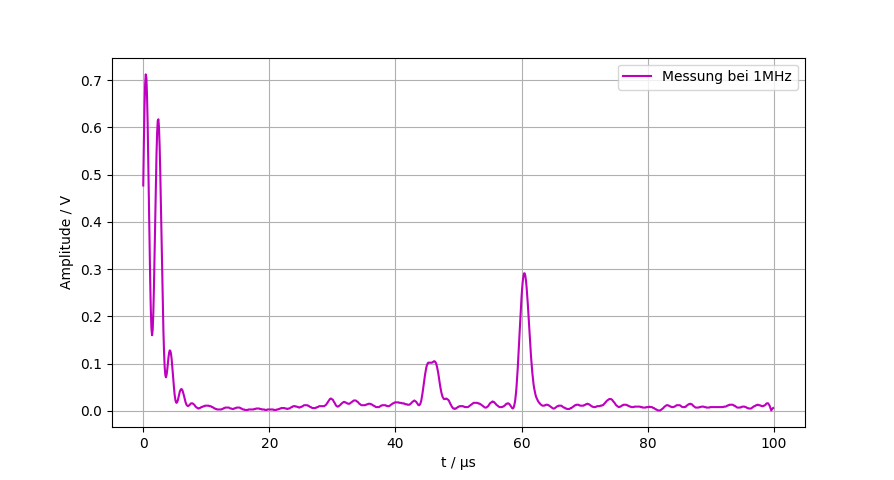
\includegraphics[width = \textwidth]{content/1mhz_aufl_plot.png}
  \caption{Die Signalamplitude in Abhängigkeit von der Laufzeit des Impulses.}
  \label{fig:1mhz}
\end{figure}
Die erhöhte Amplitude ist auch in der \autoref{fig:2mhz}, die dem B-Scan im folgenden Abschnitt entstammt, zu sehen. Das Signal der beiden kleinsten Löcher 
ist dort im Bereich von $t \approx 18\mu$s zu erkennen. 
Seine Amplitude liegt mit $U_{\mathrm{2MHz}} \approx 0,17$V deutlich über der des 1MHz-Scans $U_{\mathrm{1MHz}} \approx 0,1$V.



\begin{figure}[H]
  \centering
  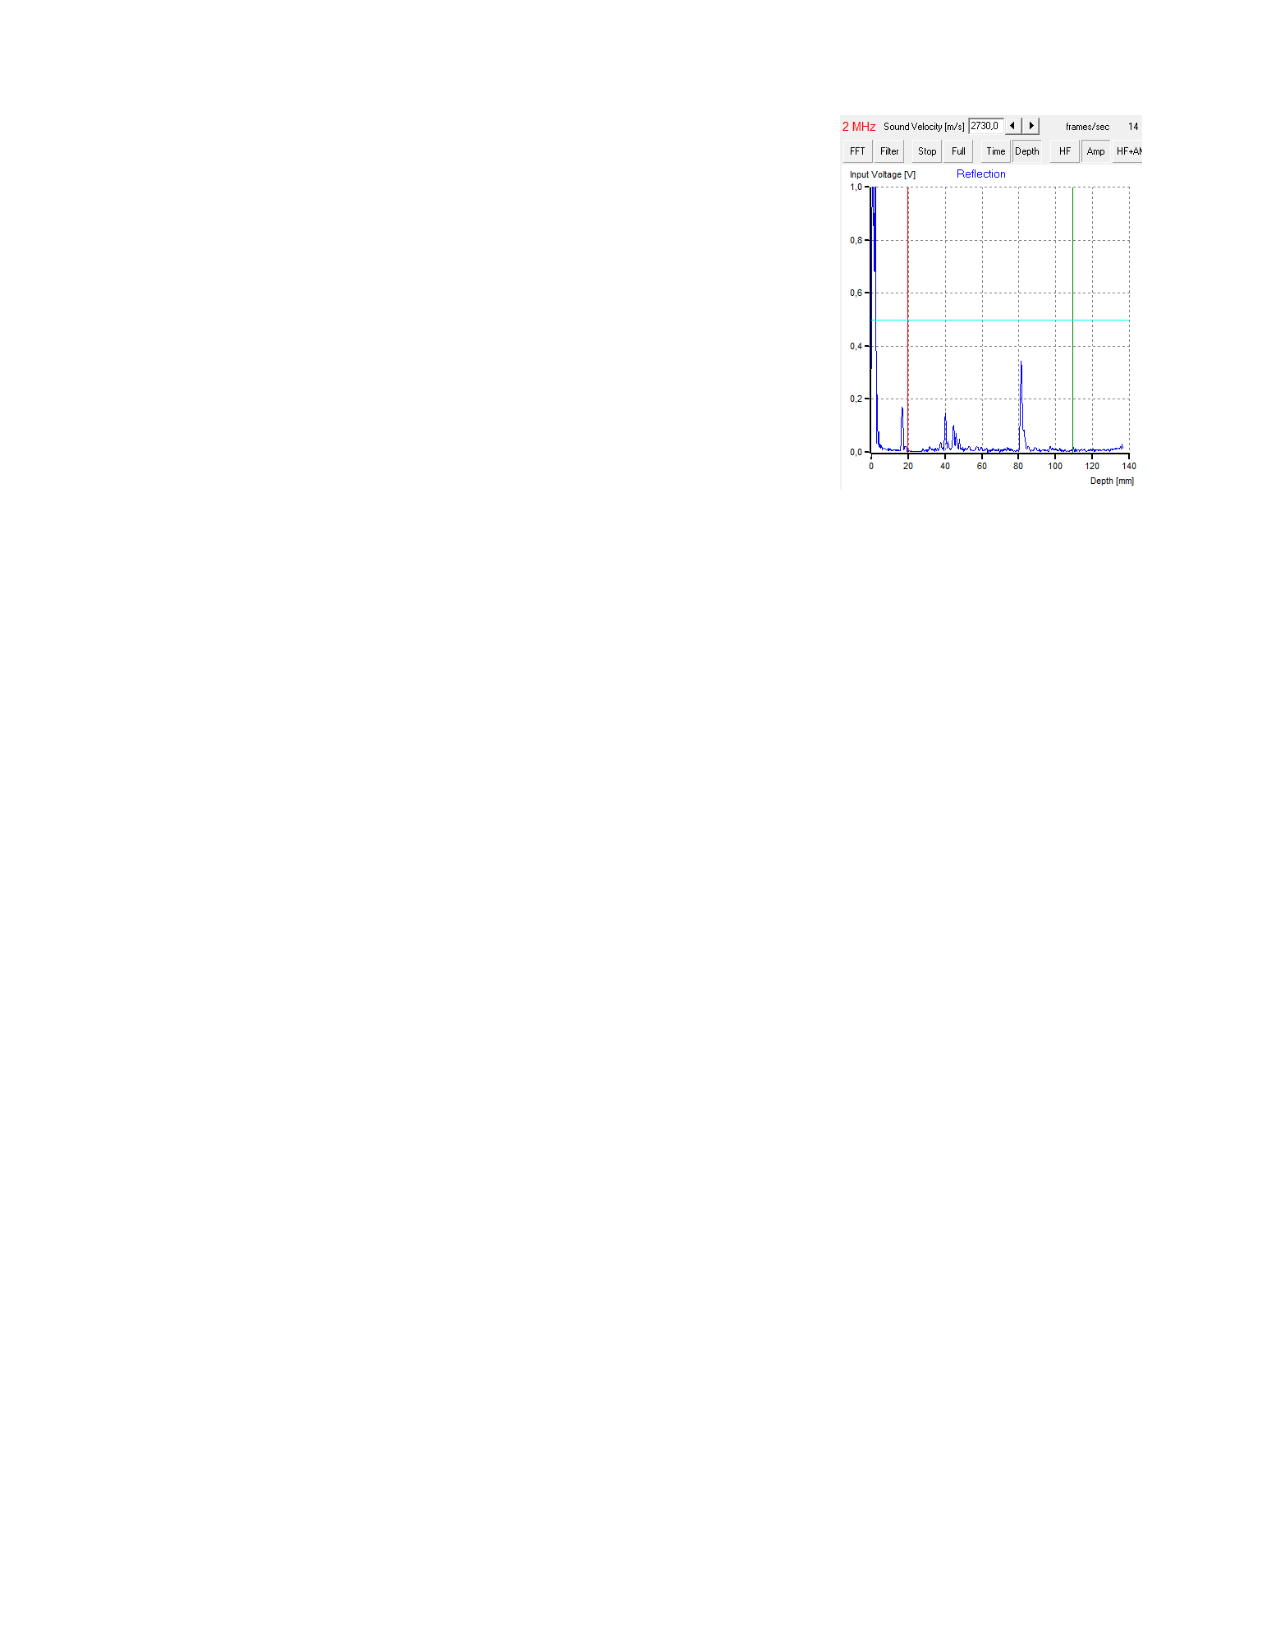
\includegraphics[width = \textwidth]{content/2Mhz.pdf}
  \caption{Die Signalamplitude in Abhängigkeit von der Laufzeit des Impulses.}
  \label{fig:2mhz}
\end{figure}


\subsection{Untersuchung eines Acrylblocks mit einem B-Scan}




\begin{figure}[H]
  \centering
  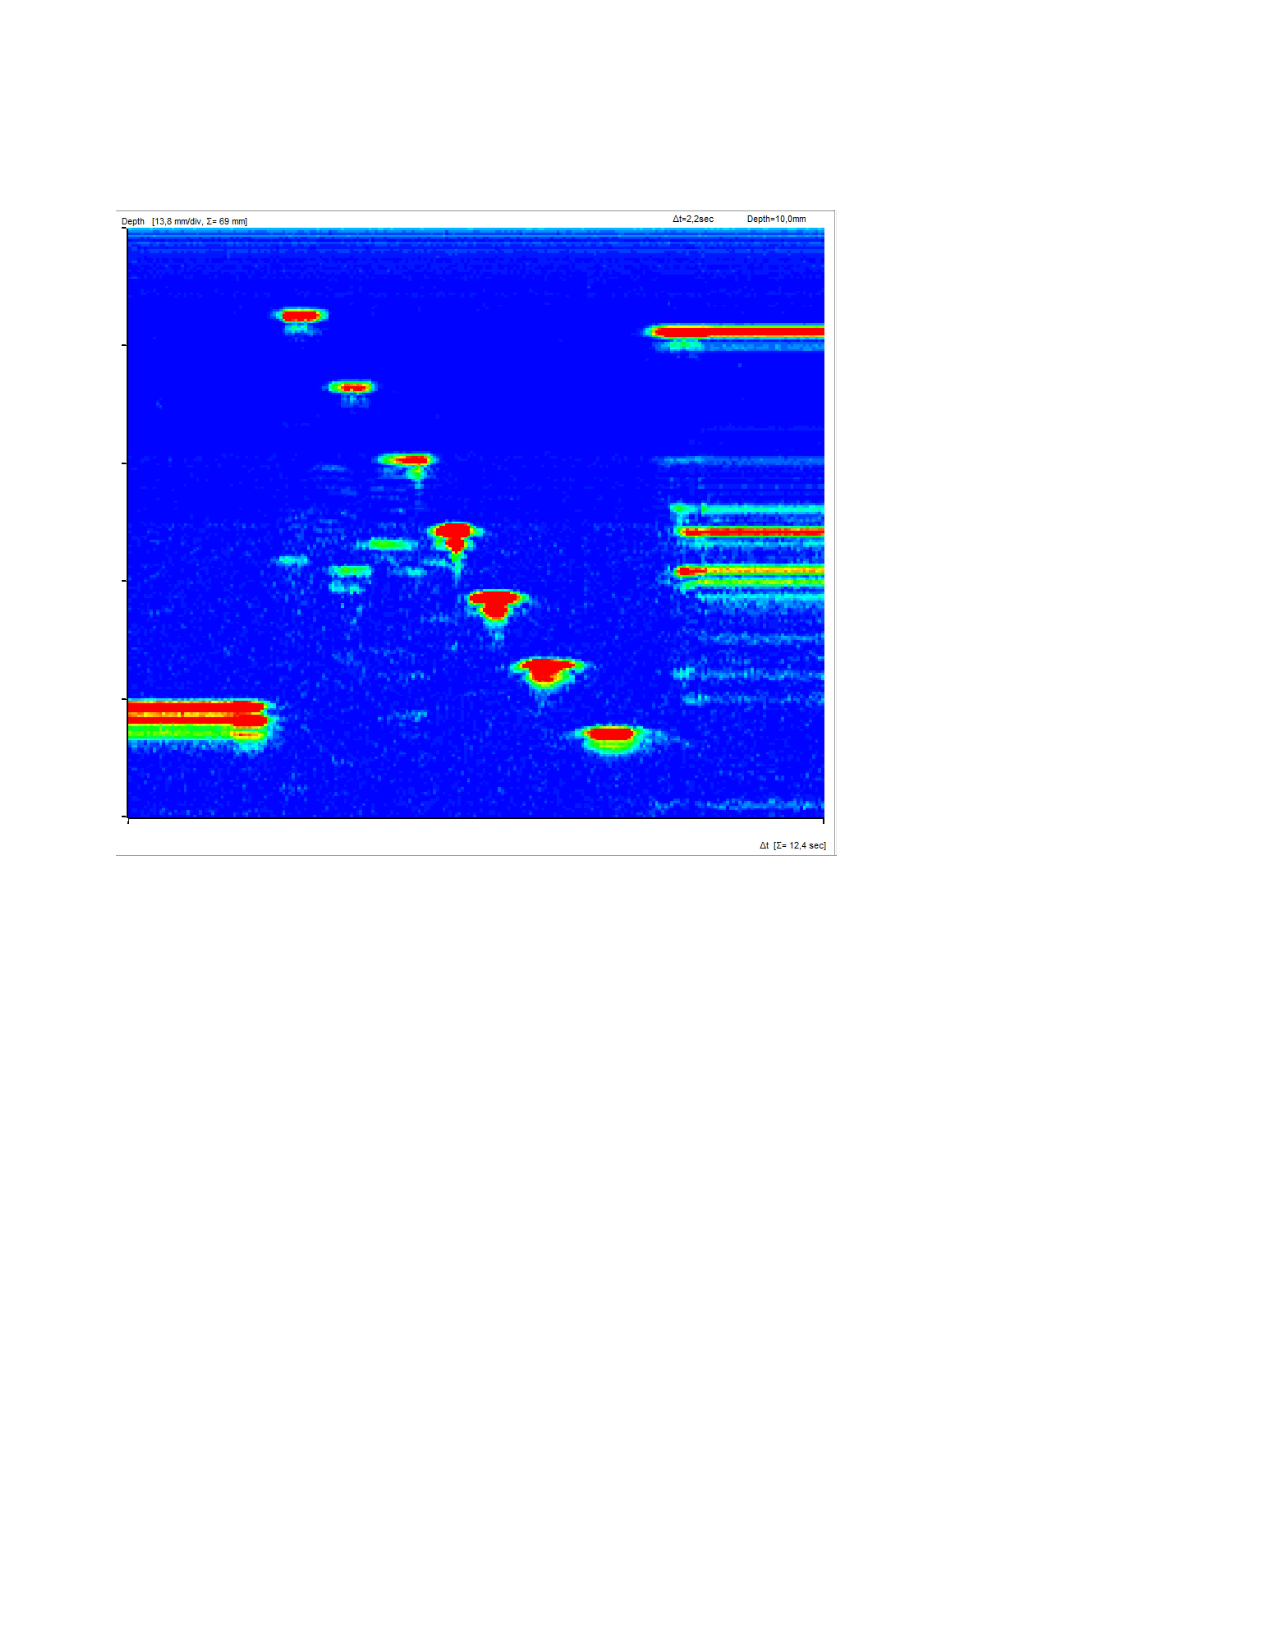
\includegraphics[width = 7cm]{content/bscan_oben.pdf}
  \caption{Die graphische Darstellung eines B-Scans des Acrylblocks von oben.}
  \label{fig:boben}
\end{figure}

\begin{figure}[H]
  \centering
  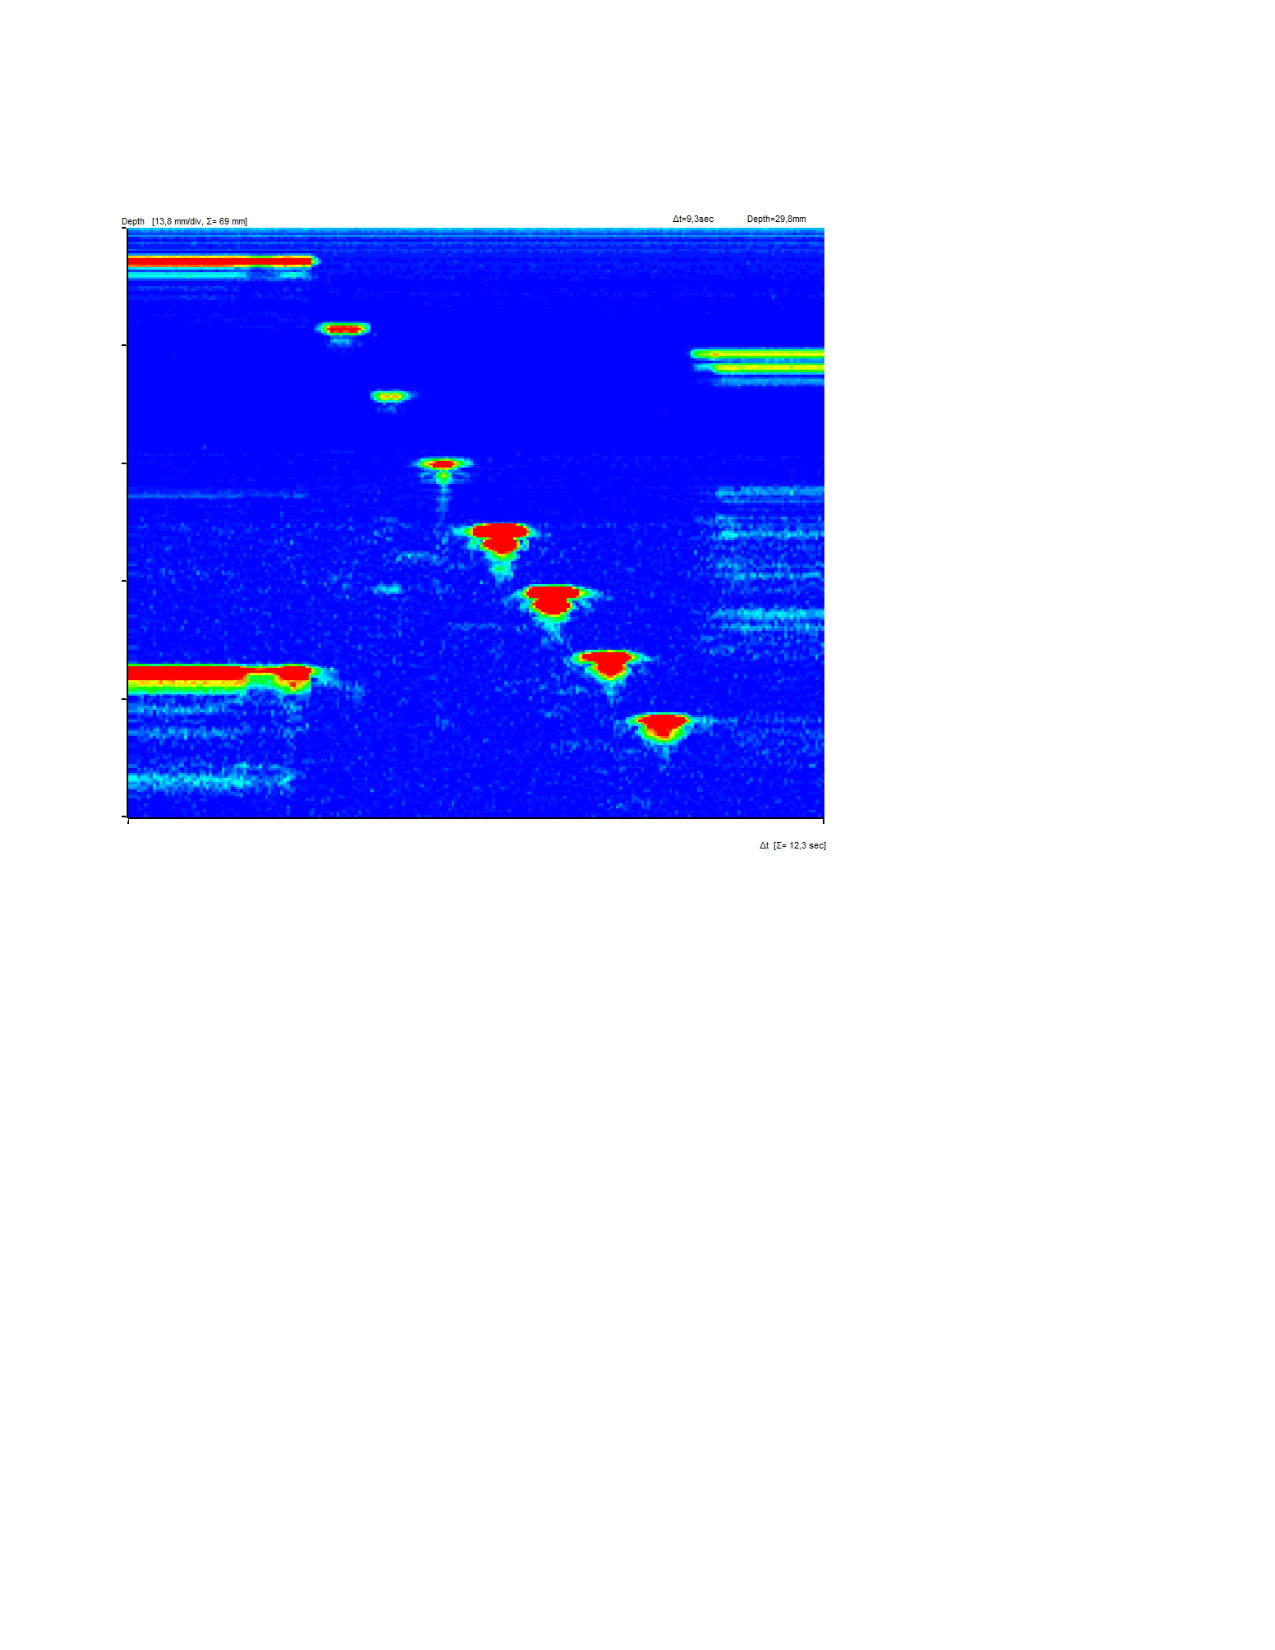
\includegraphics[width = 7cm]{content/bscan_unten.pdf}
  \caption{Die graphische Darstellung eines B-Scans des Acrylblocks von unten.}
  \label{fig:bunten}
\end{figure}


\subsection{Untersuchung eines Brustmodells mit einem B-Scan}
Beim Abtasten lässt sich die grobe Lage der Tumore ausfindig machen. \\
Einer liegt bei frontaler Betrachtung unten rechts, der andere ungefähr mittig im Modell.

\begin{figure}[H]
  \centering
  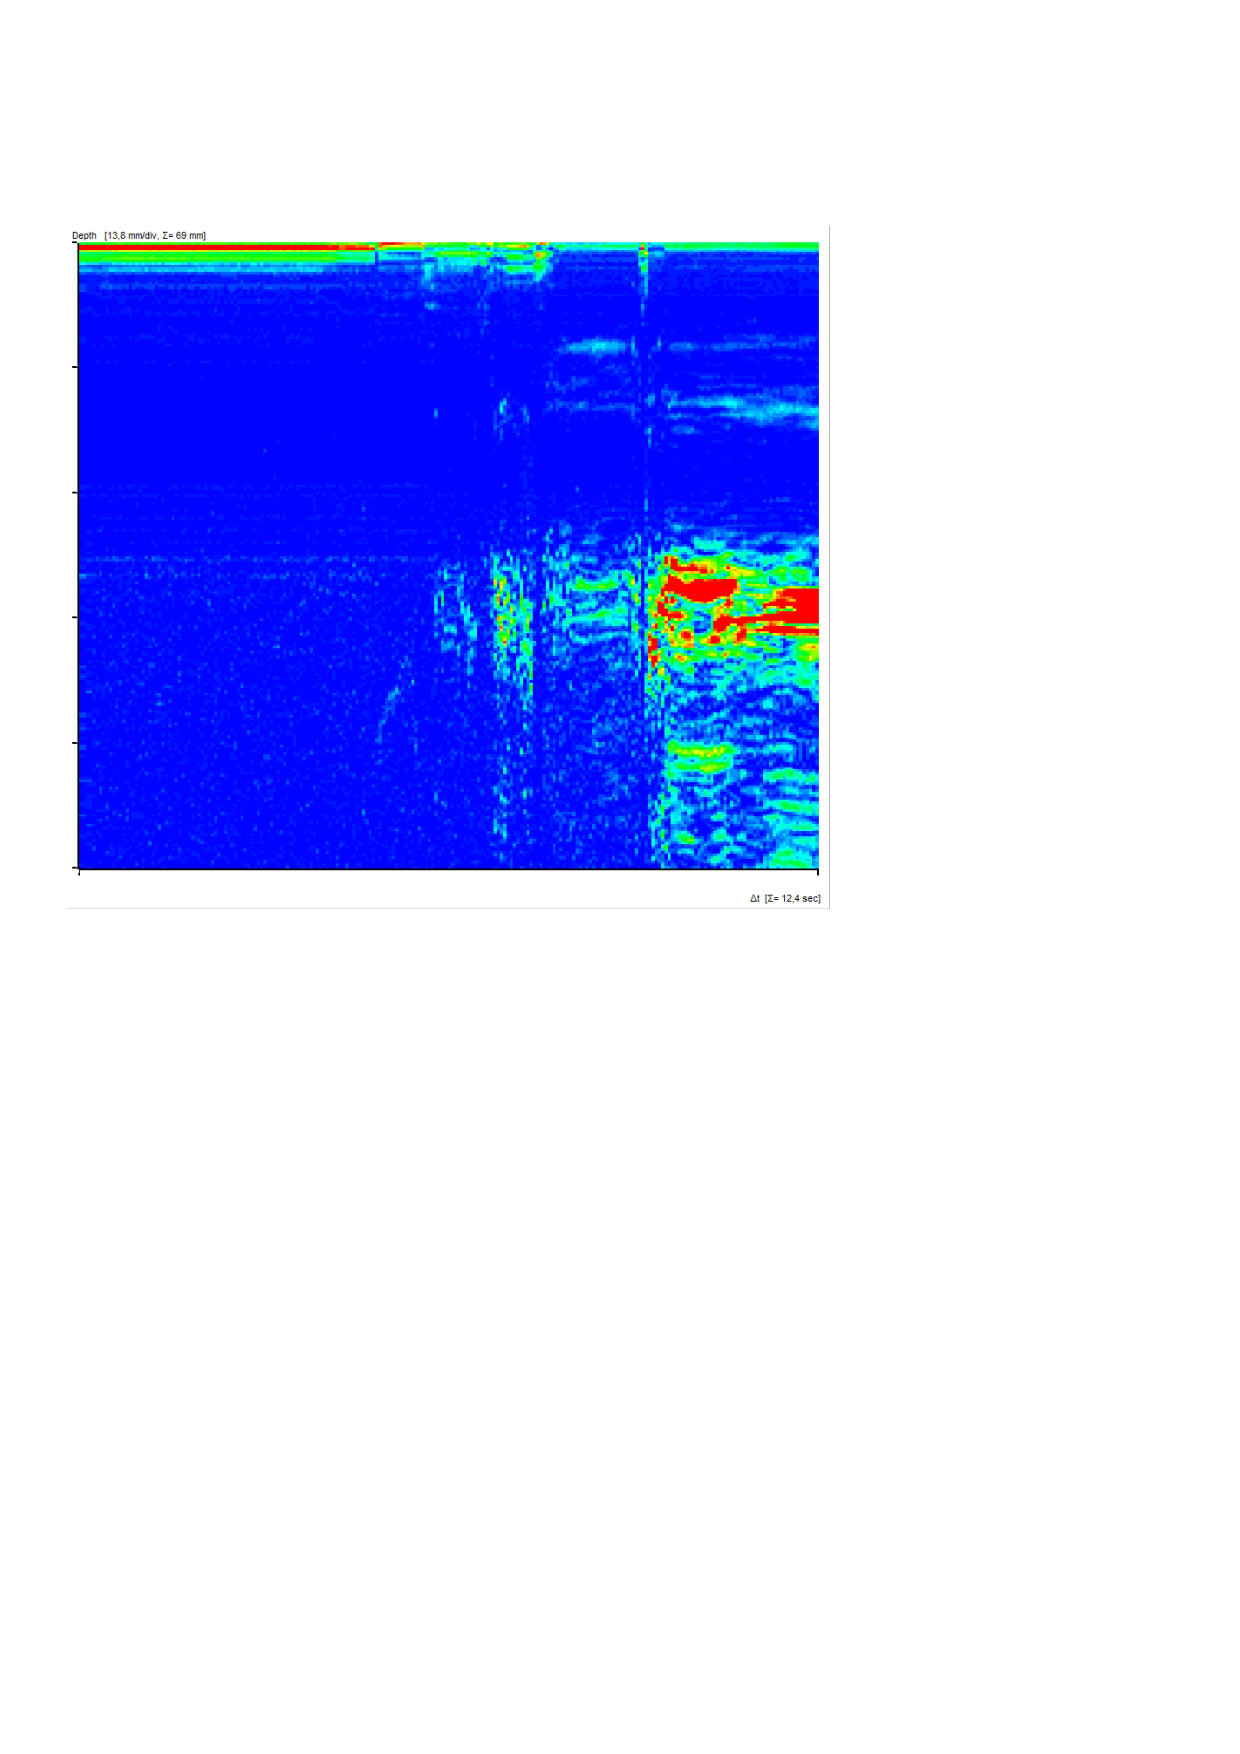
\includegraphics[width = 8cm]{content/festtumor.pdf}
  \caption{B-Scan des festen Tumors im Brustmodell.}
  \label{fig:tumorfest}
\end{figure}
\begin{figure}[H]
  \centering
  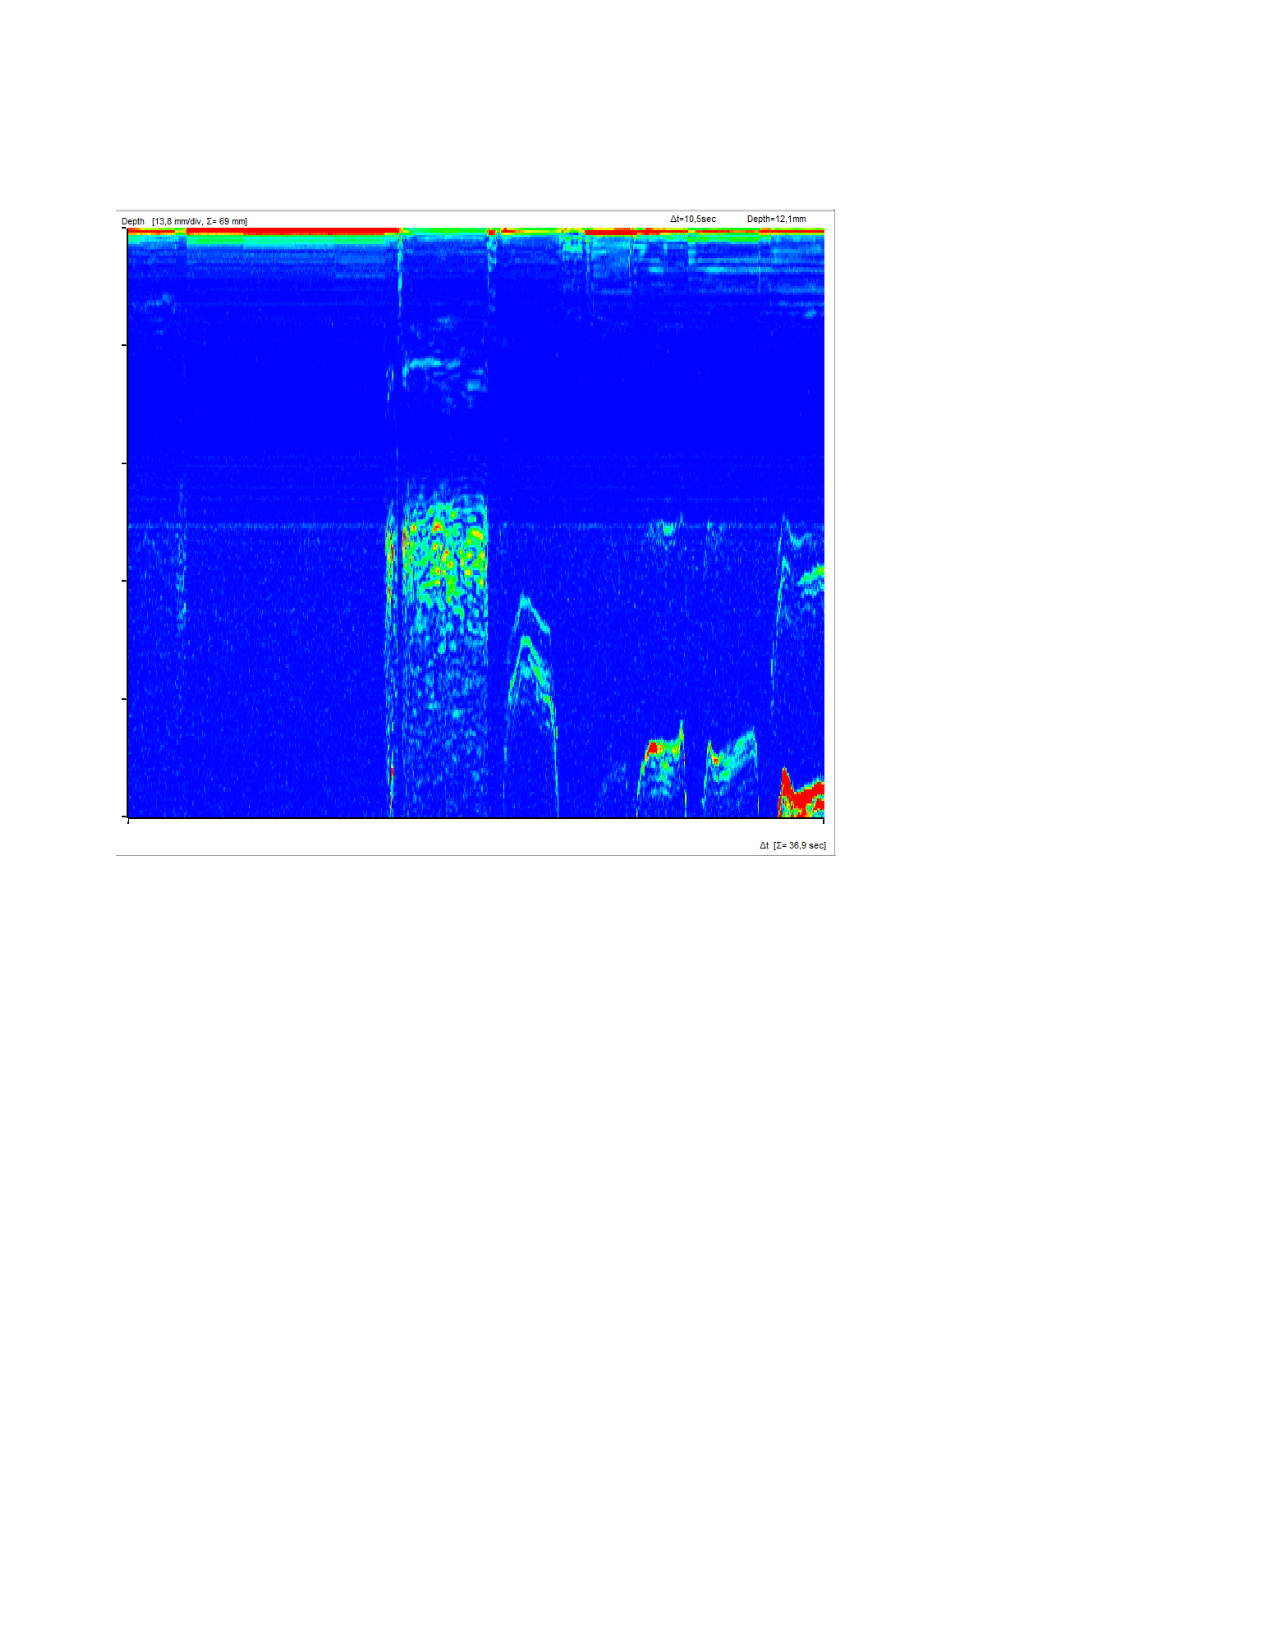
\includegraphics[width = 8cm]{content/wassertumor.pdf}
  \caption{B-Scan des flüssigkeitsgefüllten Tumors im Brustmodell.}
  \label{fig:tumorfluessig}
\end{figure}

In \autoref{fig:tumorfest} und \autoref{fig:tumorfluessig} ist deutlich der Unterschied 
in der Amplitude der vom flüssigkeitsgefüllten bzw. festen Tumor reflektierten Signals zu sehen.
Das Signal des festen Tumors in \autoref{fig:tumorfest} hat eine höhere 
Amplitude. \\
Außerdem geben die B-Scans Aufschluss über die Tiefe und den Durchmesser der Tumore.
Der feste Tumor verfügt über einen Durchmesser von xxx und liegt xxx tief.
Der Flüssige misst $d = xxx$ und liegt xxx tief im Modell.
